% ----------------------------------------------------------------------
% Set the document class
% ----------------------------------------------------------------------
\documentclass[12pt]{article}

% ----------------------------------------------------------------------
% Define external packages, language, margins, fonts, new commands 
% and colors
% ----------------------------------------------------------------------
\usepackage[utf8]{inputenc} % Codification
\usepackage[english]{babel} % Writing idiom

\usepackage{booktabs}

\usepackage[export]{adjustbox} % Align images
\usepackage{amsmath} % Extra commands for math mode
\usepackage{amssymb} % Mathematical symbols
\usepackage{anysize} % Personalize margins
    \marginsize{2cm}{2cm}{2cm}{2cm} % {left}{right}{above}{below}
\usepackage{appendix} % Appendices
\usepackage{cancel} % Expression cancellation
\usepackage{caption} % Captions
    \captionsetup{labelfont={bf}}
\usepackage{cite} % Citations, like [1 - 3]
\usepackage{color} % Text coloring
\usepackage{fancyhdr} % Head note and footnote
    \pagestyle{fancy}
    \fancyhf{}
    \fancyhead[L]{\footnotesize IST} % Left of Head note
    \fancyhead[R]{\footnotesize ULisboa} % Right of Head note
    \fancyfoot[L]{\footnotesize Traffic Engineering} % Left of Footnote
    \fancyfoot[C]{\thepage} % Center of Footnote
    \fancyfoot[R]{\footnotesize METI} % Right of Footnote
    \renewcommand{\footrulewidth}{0.4pt} % Footnote rule
\usepackage{float} % Utilization of [H] in figures
\usepackage{graphicx} % Figures in LaTeX
\usepackage[colorlinks = true, plainpages = true, linkcolor = istblue, urlcolor = istblue, citecolor = istblue, anchorcolor = istblue]{hyperref}
\usepackage{indentfirst} % First paragraph
\usepackage[super]{nth} % Superscripts
\usepackage{siunitx} % SI units
\usepackage{subcaption} % Subfigures
\usepackage{booktabs} % Professional tables
\usepackage{multirow} % Multi-row tables
\usepackage{titlesec} % Font
    \titleformat{\section}{\Large\bfseries}{\thesection}{1em}{}
    \titleformat{\subsection}{\large\bfseries}{\thesubsection}{1em}{}
    \titleformat{\subsubsection}{\normalsize\bfseries}{\thesubsubsection}{1em}{}
    \fancyfoot[C]{\thepage}

% Random text (not needed)
\usepackage{lipsum}
\usepackage{duckuments}

% New and re-newcommands
\newcommand{\sen}{\operatorname{\sen}} % Sine function definition
\newcommand{\HRule}{\rule{\linewidth}{0.5mm}} % Specific rule definition
\renewcommand{\appendixpagename}{\LARGE Appendices}

% Colors
\definecolor{istblue}{RGB}{3, 171, 230}
\definecolor{dkgreen}{rgb}{0,0.6,0}
\definecolor{gray}{rgb}{0.5,0.5,0.5}

%%%%%%%%%%%%%%%%%%%%%%%%%%%%%%%%%%%%%%%%%%%%%%%%%%%%%%%%%%%%%%%%%%%%%%%%
%                                 Document                             %
%%%%%%%%%%%%%%%%%%%%%%%%%%%%%%%%%%%%%%%%%%%%%%%%%%%%%%%%%%%%%%%%%%%%%%%%
\begin{document}

% ----------------------------------------------------------------------
% Cover
% ----------------------------------------------------------------------
\begin{center}
    \begin{figure}
        \vspace{-1.0cm}
        
\includegraphics[scale = 0.25, left]{Images/IST_A.png} % IST logo
    \end{figure}
    \mbox{}\\[2.0cm]
    \textsc{\Huge Traffic Engineering}\\[2.5cm]
    \textsc{\LARGE METI}\\[2.0cm]
    \HRule\\[0.4cm]
    {\large \bf {Lab 1 Report} [\texttt{EN}]}\\[0.2cm]
    \HRule\\[1.5cm]
\end{center}

\begin{flushleft}
    \textbf{Authors:}
\end{flushleft}

\begin{center}
    \begin{minipage}{0.5\textwidth}
        \begin{flushleft}
            José Oliveira (103771)\\
            Tiago Videira (116069)\\
        \end{flushleft}
    \end{minipage}%
    \begin{minipage}{0.5\textwidth}
        \begin{flushright}
            \href{mailto:jose.novais.oliveira@tecnico.ulisboa.pt}{\texttt{jose.novais.oliveira@tecnico.ulisboa.pt}}\\
            \href{mailto:tiago.g.videira@tecnico.ulisboa.pt}{\texttt{tiago.g.videira@tecnico.ulisboa.pt}}\\
        \end{flushright}
    \end{minipage}
\end{center}
    
\begin{flushleft}
    \large $\boxed{\text{\bf Group 5}}$\\[4.0cm]
\end{flushleft}
    
\begin{center}
    \large \bf 2025/2026 -- \nth{2} Semester, P4
\end{center}

\thispagestyle{empty}

\setcounter{page}{0}

\tableofcontents
\newpage

\newpage

\section{Introduction}

The objective of this laboratory assignment is to simulate and analyse stochastic processes commonly used to model traffic in communication networks.

The work developed in this assignment includes:

\begin{itemize}
    \item Simulation of Poisson arrival processes and comparison with the theoretical distribution;
    \item Analysis of the impact of different values of $\lambda$ on the behaviour of the process;
    \item Superposition of multiple independent Poisson processes and validation of their statistical properties;
    \item Simulation of an M/M/1 queue using a discrete-event approach;
    \item Evaluation of key performance metrics, including:
    \begin{itemize}
        \item Average queue length;
        \item Waiting time in the queue;
        \item Total time in the system;
        \item Server utilization;
    \end{itemize}
\end{itemize}

All simulations were implemented in Python using pseudo-random number generation and numerical methods. The results were analysed through graphical representations and comparison with theoretical models.

\newpage

\section{Poisson Process Simulation}

\subsection{Theoretical Background}

A Poisson process with parameter $\lambda$ represents a random arrival process in which the number of events occurring in a unit time interval follows a Poisson distribution:

\begin{equation}
P(X=k)=\frac{\lambda^k e^{-\lambda}}{k!}
\end{equation}

where:

\begin{itemize}
    \item $k$ = number of events in one interval;
    \item $\lambda$ = average arrival rate.
\end{itemize}

The time between two consecutive arrivals follows an exponential distribution:

\begin{equation}
f(t)=\lambda e^{-\lambda t}, \quad t \geq 0
\end{equation}

To generate exponentially distributed inter-arrival times, the inverse transform method was used:

\begin{equation}
\Delta t = \frac{-\ln(1-u)}{\lambda}
\end{equation}

where $u$ is uniformly distributed in $[0,1)$.

\subsection{Implementation Method}

For each experiment:

\begin{enumerate}
    \item Generate $N$ inter-arrival times $\Delta t$;
    \item Compute cumulative arrival instants;
    \item Divide time into unit intervals;
    \item Count the number of arrivals in each interval;
    \item Build the histogram manually;
    \item Compare experimental probabilities with the theoretical Poisson law.
\end{enumerate}

The use of built-in histogram functions was intentionally avoided, as requested in the assignment statement.

\newpage

\subsection{Results for Different Values of $\lambda$}

The simulator was executed for:

\[
\lambda = \{0.5,\;1,\;5,\;10,\;50\}
\]

For each value, the number of generated samples was increased proportionally in order to reduce statistical noise for large $\lambda$ values.

\subsubsection*{$\lambda = 0.5$}

For small values of $\lambda$, most intervals contain zero or one arrival. This behaviour matches the theoretical expectation, where $P(0)$ is dominant.

\begin{figure}[H]
    \centering
    
\includegraphics[width=0.75\textwidth]{../plots/poisson_lambda_0.5.png}
    \caption{Experimental and theoretical distribution for $\lambda=0.5$.}
\end{figure}

The probability mass remains concentrated at low values of $k$, although intervals with two or more arrivals become more frequent.

\begin{figure}[H]
    \centering
    
\includegraphics[width=0.75\textwidth]{../plots/poisson_lambda_1.0.png}
    \caption{Experimental and theoretical distribution for $\lambda=1$.}
\end{figure}

The distribution becomes wider and more symmetric around the mean value.

\begin{figure}[H]
    \centering
    
\includegraphics[width=0.75\textwidth]{../plots/poisson_lambda_5.0.png}
    \caption{Experimental and theoretical distribution for $\lambda=5$.}
\end{figure}

\begin{figure}[H]
    \centering
    
\includegraphics[width=0.75\textwidth]{../plots/poisson_lambda_10.0.png}
    \caption{Experimental and theoretical distribution for $\lambda=10$.}
\end{figure}

For very large arrival rates, the Poisson distribution becomes approximately bell-shaped due to convergence towards a normal distribution.

\begin{figure}[H]
    \centering
    
\includegraphics[width=0.75\textwidth]{../plots/poisson_lambda_50.0.png}
    \caption{Experimental and theoretical distribution for $\lambda=50$.}
\end{figure}

\newpage

\subsection{Discussion}

The obtained results validate the simulator implementation. As the number of generated events increases, the experimental distribution converges to the theoretical model.

It was also observed that:

\begin{itemize}
    \item Small $\lambda$ values produce sparse arrival patterns;
    \item Larger $\lambda$ values generate more regular and concentrated distributions;
    \item Increasing the sample size improves accuracy and reduces random fluctuations.
\end{itemize}

\section{Superposition of Poisson Processes}

\subsection{Theoretical Background}

A fundamental property of Poisson processes states that the superposition of independent Poisson processes is also a Poisson process whose rate is equal to the sum of the individual rates.

Given four independent processes:

\[
\lambda_1=2,\quad
\lambda_2=9,\quad
\lambda_3=11,\quad
\lambda_4=15
\]

the resulting combined process has parameter:

\begin{equation}
\lambda_{total}=2+9+11+15=37
\end{equation}

\subsection{Implementation}

Four independent Poisson processes were generated using exponential inter-arrival times with parameters $\lambda_1, \lambda_2, \lambda_3,$ and $\lambda_4$. 

Instead of fixing a predefined number of events for each process, all processes were simulated over a common observation interval $T$. This approach ensures that the resulting number of events in each process is consistent with the statistical properties of a Poisson process, where the number of arrivals in a time interval is itself a random variable.

The choice of a fixed observation interval is essential for correctly demonstrating the superposition property. In a Poisson process, the expected number of arrivals in a time interval $T$ is given by:

\[
\mathbb{E}[N(T)] = \lambda T
\]

Thus, for each individual process, the number of generated events naturally depends on both the rate $\lambda$ and the observation interval $T$. Processes with higher $\lambda$ values produce, on average, more events within the same interval.

After generating the four independent arrival sequences over the same interval $T$, their arrival instants were merged into a single sequence and sorted in chronological order. This produces a valid combined arrival process.

A histogram of the number of events per unit time interval was then constructed using the same methodology described in Section 2.2. This histogram was compared against the theoretical Poisson distribution with parameter:

\[
\lambda_{total} = \sum_i \lambda_i
\]

\subsection{Results}

In practice, a fixed number of events $N$ was generated for each process, which implicitly defines a random observation interval $T$. For sufficiently large $N$, this approach provides a good approximation of a Poisson process observed over a fixed time window.

\begin{figure}[H]
    \centering
    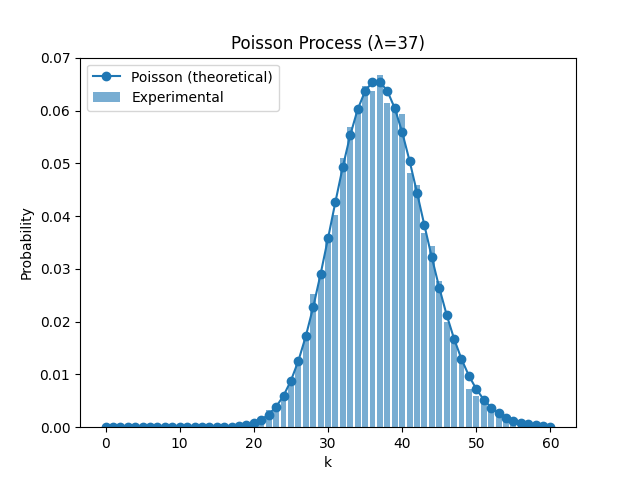
\includegraphics[width=0.8\textwidth]{../plots/superposition_lambda_37.png}
    \caption{Experimental and theoretical distribution for the superposed process ($\lambda=37$).}
\end{figure}

The experimental histogram is centered near the expected mean value and follows the theoretical Poisson distribution with good accuracy.

\subsection{Discussion}

This experiment confirms the closure property of Poisson processes under superposition. The sum of independent arrival streams preserves the Poisson nature of the process while increasing the global arrival rate.

Such behaviour is highly relevant in communication networks, where traffic generated by multiple independent users can often be modelled as a single aggregate Poisson flow.

\newpage

\section{M/M/1 Queue Simulation}

\subsection{Theoretical Background}

An M/M/1 queue models a system with Poisson arrivals and exponentially distributed service times, processed by a single server operating under a FIFO discipline.

The key parameter of the system is the utilization factor:

\begin{equation}
\rho = \frac{\lambda}{\mu}
\end{equation}

The behaviour of the system depends on $\rho$:

\begin{itemize}
    \item $\rho < 1$: stable system;
    \item $\rho = 1$: critical regime;
    \item $\rho > 1$: unstable system.
\end{itemize}

For a stable system, the theoretical performance metrics are:

\begin{equation}
L_q = \frac{\rho^2}{1 - \rho}
\end{equation}

\begin{equation}
W_q = \frac{\rho}{\mu - \lambda}
\end{equation}

\begin{equation}
W = \frac{1}{\mu - \lambda}
\end{equation}

\begin{equation}
U = \rho
\end{equation}

\subsection{Implementation Method}

The M/M/1 queue was simulated using a discrete-event approach, where events correspond to packet arrivals and departures.

Inter-arrival times were generated using an exponential distribution with parameter $\lambda$. This was implemented using the inverse transform method:

\begin{equation}
\Delta t = \frac{-\ln(1-u)}{\lambda}
\end{equation}

where $u$ is a uniformly distributed random variable in $[0,1)$.

Similarly, service times were generated using an exponential distribution with parameter $\mu$:

\begin{equation}
S = \frac{-\ln(1-u)}{\mu}
\end{equation}

The system state was updated by processing events in chronological order. At each step, the simulation clock advanced to the next event time.

The queue was implemented as a FIFO structure storing arrival instants, allowing the computation of waiting time:

\begin{equation}
W_q = t_{start} - t_{arrival}
\end{equation}

and total system time:

\begin{equation}
W = W_q + S
\end{equation}

Time-dependent performance metrics were computed using time averages. The average queue length was obtained by integrating the queue size over time:

\begin{equation}
L_q = \frac{1}{T} \int_0^T Q(t)\,dt
\end{equation}

Similarly, server utilization was computed as:

\begin{equation}
U = \frac{1}{T} \int_0^T B(t)\,dt
\end{equation}

where $Q(t)$ represents the queue size and $B(t)$ indicates whether the server is busy.

\subsection{Queue Evolution Over Time}

The evolution of the queue size was analysed for increasing numbers of simulated events.

\begin{figure}[H]
\centering

\begin{subfigure}{0.32\textwidth}
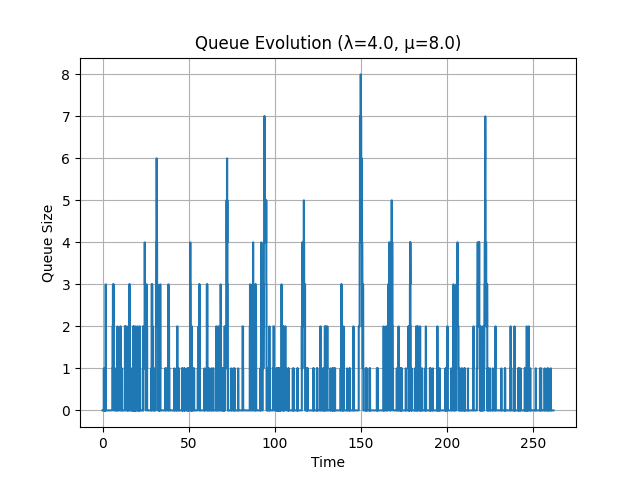
\includegraphics[width=\linewidth]{../queue_lambda_4.0_mu_8.0_1000.png}
\caption{1000 events}
\end{subfigure}
\hfill
\begin{subfigure}{0.32\textwidth}
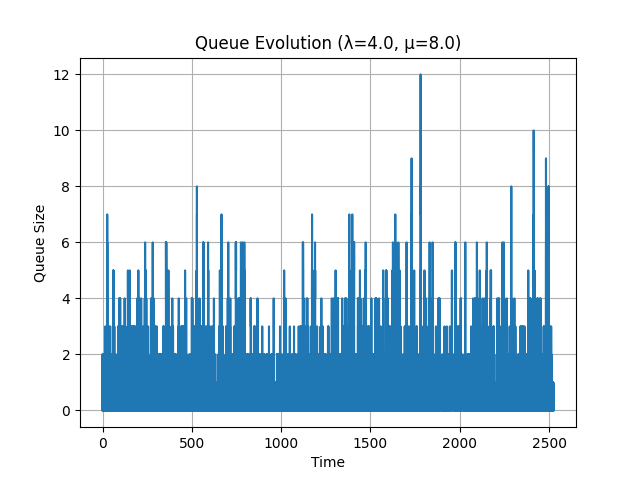
\includegraphics[width=\linewidth]{../queue_lambda_4.0_mu_8.0_10000.png}
\caption{10000 events}
\end{subfigure}
\hfill
\begin{subfigure}{0.32\textwidth}
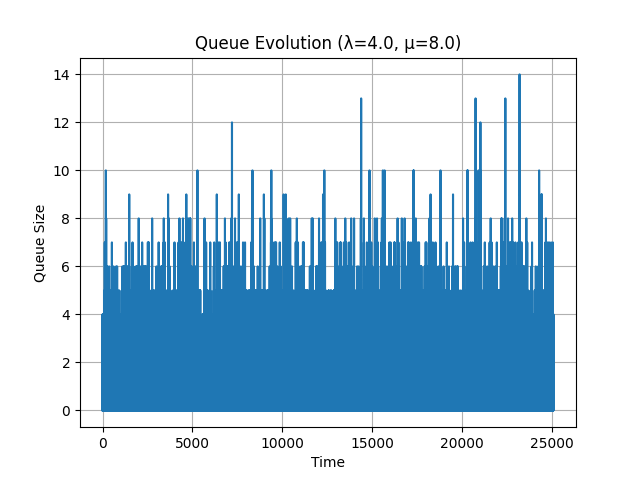
\includegraphics[width=\linewidth]{../queue_lambda_4.0_mu_8.0_100000.png}
\caption{100000 events}
\end{subfigure}

\caption{Queue evolution over time for increasing number of simulated events ($\lambda=4$, $\mu=8$)}
\end{figure}

It can be observed that as the number of simulated events increases, the queue behaviour becomes more stable and starts to ressemble the expected theoretical behaviour of an M/M/1 queue with $\rho=0.5$.

\subsection{Comparison with Theoretical Results}

\begin{table}[H]
\centering
\begin{tabular}{ccccc}
\toprule
Events & $L_q$ & $\rho$ & $W_q$ & $W$ \\
\midrule
1000   & 0.364 & 0.462 & 0.096 & 0.217 \\
10000  & 0.540 & 0.507 & 0.133 & 0.259 \\
100000 & 0.497 & 0.499 & 0.125 & 0.250 \\
\midrule
Theory & 0.500 & 0.500 & 0.125 & 0.250 \\
\bottomrule
\end{tabular}
\caption{Simulation vs theoretical results for $\lambda=4$, $\mu=8$}
\end{table}

The results show a clear convergence towards theoretical values as the number of events increases.

For a small number of events, the estimates present higher variability due to randomness. However, as the number of events increases, the simulation becomes more accurate and approaches the expected theoretical behaviour.

\subsection{Queue Behaviour Under Different Regimes}

In addition to validating the simulator, the behaviour of the system under different operating conditions was analysed.

\begin{figure}[H]
\centering

\begin{subfigure}{0.32\textwidth}
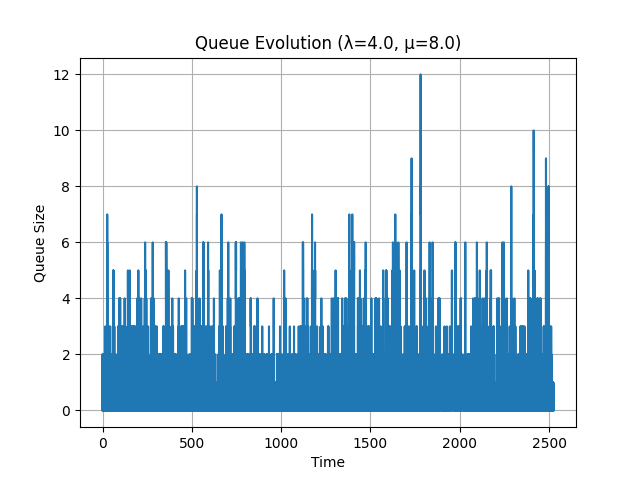
\includegraphics[width=\linewidth]{../queue_lambda_4.0_mu_8.0_10000.png}
\caption{$\lambda < \mu$}
\end{subfigure}
\hfill
\begin{subfigure}{0.32\textwidth}
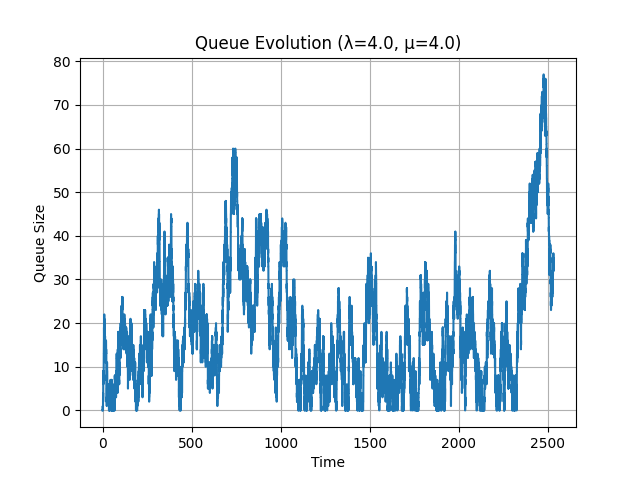
\includegraphics[width=\linewidth]{../queue_lambda_4.0_mu_4.0_10000.png}
\caption{$\lambda = \mu$}
\end{subfigure}
\hfill
\begin{subfigure}{0.32\textwidth}
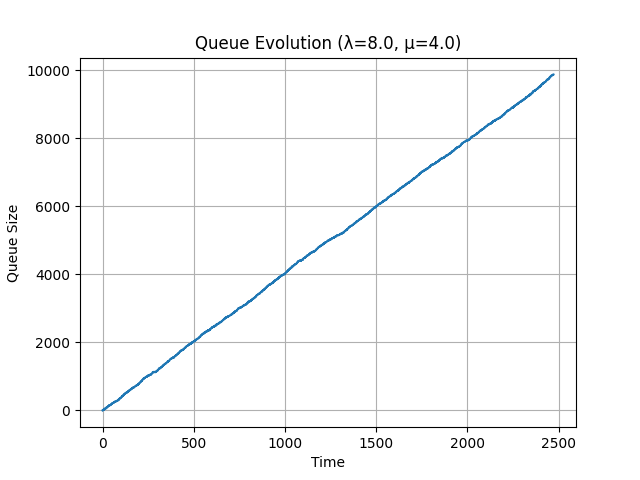
\includegraphics[width=\linewidth]{../queue_lambda_8.0_mu_4.0_10000.png}
\caption{$\lambda > \mu$}
\end{subfigure}

\caption{Queue evolution for different operating regimes}
\end{figure}

The behaviour of the queue depends strongly on the relationship between the arrival rate $\lambda$ and the service rate $\mu$.

For $\lambda < \mu$, the queue remains stable and fluctuates around a finite value.

For $\lambda = \mu$, the system operates at the stability limit and the queue exhibits a growing trend.

For $\lambda > \mu$, the queue grows rapidly over time, indicating an unstable system.

\subsection{Discussion}

The simulation results confirm the theoretical behaviour of M/M/1 queueing systems.

In the stable regime, the system reaches equilibrium and the measured metrics closely match theoretical predictions.

As the system approaches the critical regime, performance degrades significantly, with increasing queue lengths and delays.

In the unstable regime, the divergence of the queue highlights the importance of maintaining a service rate higher than the arrival rate in practical systems.

These results demonstrate the fundamental relationship between system load and performance in queueing systems.

\newpage

\section{Conclusion}

This laboratory work successfully explored the properties of Poisson arrival processes and their application to queueing systems.

The simulation of Poisson processes demonstrated a strong agreement between experimental results and the theoretical distribution. The impact of the parameter $\lambda$ on the shape and dispersion of the distribution was clearly observed.

The superposition experiment confirmed that the aggregation of independent Poisson processes results in another Poisson process, with rate equal to the sum of the individual rates.

The M/M/1 queue simulation further extended this analysis by introducing service dynamics. The results showed that system performance strongly depends on the relationship between arrival and service rates.

In particular:
\begin{itemize}
    \item For $\lambda < \mu$, the system remains stable and performance metrics converge to theoretical values;
    \item For $\lambda = \mu$, the system operates at the stability limit;
    \item For $\lambda > \mu$, the system becomes unstable and the queue grows without bound.
\end{itemize}

Overall, the results highlight the importance of maintaining adequate service capacity in systems subject to stochastic traffic, such as communication networks.


\end{document}
